
\section{Derivation of the time dilation formula within VAM}\label{sec:appendix:1}

\begin{abstract}
We present a unified time dilation formula derived from the Vortex \AE{}ther Model (VAM), a fluid-dynamic reformulation of gravitation and mass-energy interactions. Unlike General Relativity, where mass and curvature govern clock rates, VAM attributes gravitational phenomena to quantized vorticity, æther circulation, and swirl-induced pressure gradients. The proposed equation replaces the Schwarzschild and Kerr metric terms with vortex core tangential velocities, swirl angular frequencies, and an effective mass derived from exponentially decaying æther density. A hybridization mechanism smoothly interpolates between vortex-scale gravity and classical Newtonian coupling at macroscopic distances. The final expression captures six physical effects within one coherent framework: (1) vortex-induced mass generation via circulation and helicity, (2) bubble-like volume expansion due to internal irrotational flow, (3) acceleration of this flow under compression, (4) thermal-like energy response from swirl speedup, (5) relativistic time dilation from æther puncture during motion, and (6) swirl-based core-local time. The result is a mathematically robust, numerically testable model that unifies quantum vortex dynamics with gravitational time effects and remains non-singular across all radial domains.
\end{abstract}

\section*{Introduction}
In General Relativity (GR), time dilation is sourced by mass and rotation via the Schwarzschild and Kerr metrics, respectively. The Vortex \ae{}ther Model (VAM) replaces these with swirl-induced vorticity, æther density gradients, and circulation fields. We derive and present a unified time dilation expression that incorporates:

\begin{itemize}
    \item Vortex-induced mass formation,
    \item Frame-dragging via swirl angular velocity,
    \item Bubble swelling dynamics mimicking thermodynamic gas laws,
    \item Exponential decay of æther vorticity with distance,
    \item Hybridization to classical GR at large $r$.
\end{itemize}

\subsection{Final VAM Time Dilation Equation}
The unified time dilation equation in VAM becomes, expressed as the ratio between local Chronos-Time $\tau$ and global Aithēr-Time $\mathcal{N}$:

\begin{equation}
\boxed{
\frac{d\tau}{d\mathcal{N}} = \sqrt{
1
- \frac{2 G_{\text{hybrid}}(r) M_{\text{hybrid}}(r)}{r c^2}
- \frac{C_e^2}{c^2} e^{-r/r_c}
- \frac{C_e^2}{r_c^2 c^2} e^{-r/r_c}
}}
\label{eq:final_vam_td}
\end{equation}
Here, $\tau$ is the local proper time tracked by a particle in the vortex region (Chronos-Time), and $\mathcal{N}$ is the background causal time of the æther (Aithēr-Time).

$\frac{d\tau}{dt} = \sqrt{
1
- \frac{C_e^2}{c^2} e^{-r/r_c}
- \frac{2G_\text{swirl} M_\text{eff}(r)}{r c^2}
- \beta \Omega^2
}$

Uses standard coordinate time $t$, not the universal Aithēr-Time $\mathcal{N}$.

\subsection{Explanation of Terms}

Each term represents a physical mechanism:

\begin{itemize}
  \item \textbf{Term 1: Core rotation (local swirl)}
  \[
    \frac{C_e^2}{c^2} e^{-r/r_c}
  \]
  This term is derived from the intrinsic angular velocity $\Omega_\text{core}$ of the vortex core. The tangential velocity $C_e$ is the maximum swirl at the core boundary, and $r_c$ is the radius of the vortex core. The exponential factor $e^{-r/r_c}$ represents the decrease in influence at distance $r$ outside the core. This term represents the time delay due to local æther rotation.

  \item \textbf{Term 2: Gravitational field (vorticity-induced potential)}
  \[
    \frac{2 G_\text{swirl} M_\text{eff}(r)}{r c^2}
  \]
  This term mimics the classical gravitational redshift, but with an alternative gravitational constant $G_\text{swirl}$ that follows from æther parameters such as density and swirl force. The effective mass $M_\text{eff}(r)$ can be taken here as the æther vortex energy within radius $r$, instead of conventional mass. This term arises from the pressure deficit due to external swirl and replaces Newtonian gravity.

  \item \textbf{Term 3: Macroscopic rotation (frame-dragging)}
  \[
    \beta \Omega^2
  \]
  This term represents frame-dragging effects within a rotating vortex configuration (similar to the Kerr metric effect in GR). The factor $\Omega$ is the rotation rate of the macroscopic object (e.g. planet or neutron star), and $\beta$ is a coupling constant that depends on æther parameters. The term originates from circulation energy with $\Omega = \Gamma / (2\pi r^2)$ and $\Gamma = \oint \vec{v} \cdot d\vec{\ell}$, while the coupling factor $\beta = 1/c^2$ reflects ætheric inertial drag. This yields a rotational dilation term $\beta \Omega^2 \sim \frac{C_e^2}{r_c^2 c^2} e^{-r/r_c}$. This term causes additional local time delay due to circulation of the surrounding æther field.

\end{itemize}

\subsection{Hybridization of Gravitational Coupling}

To reconcile predictions for macroscopic systems, we define:
\[
    \mu(r) = \exp\left(-\frac{r^2}{R_0^2}\right), \quad R_0 \sim 10^{-12} \, \mathrm{m}
\]
\begin{align*}
    G_{\text{hybrid}}(r) &= \mu(r) \, G_{\text{swirl}} + (1 - \mu(r)) \, G \\
    M_{\text{hybrid}}(r) &= \mu(r) \, M_{\text{eff}}^\text{VAM}(r) + (1 - \mu(r)) \, M
\end{align*}

\subsection{Effective VAM Mass}
Assuming an exponentially decaying æther density:
\[
\rho_\text{\ae}(r) = \rho_0 e^{-r / r_c}
\]
The effective mass becomes:
\[
M_\text{eff}^\text{VAM}(r) = 4\pi \rho_0 r_c^3 \left(2 - \left(2 + \frac{r}{r_c} \right) e^{-r/r_c} \right)
\]

\begin{figure}[H]
  \centering
  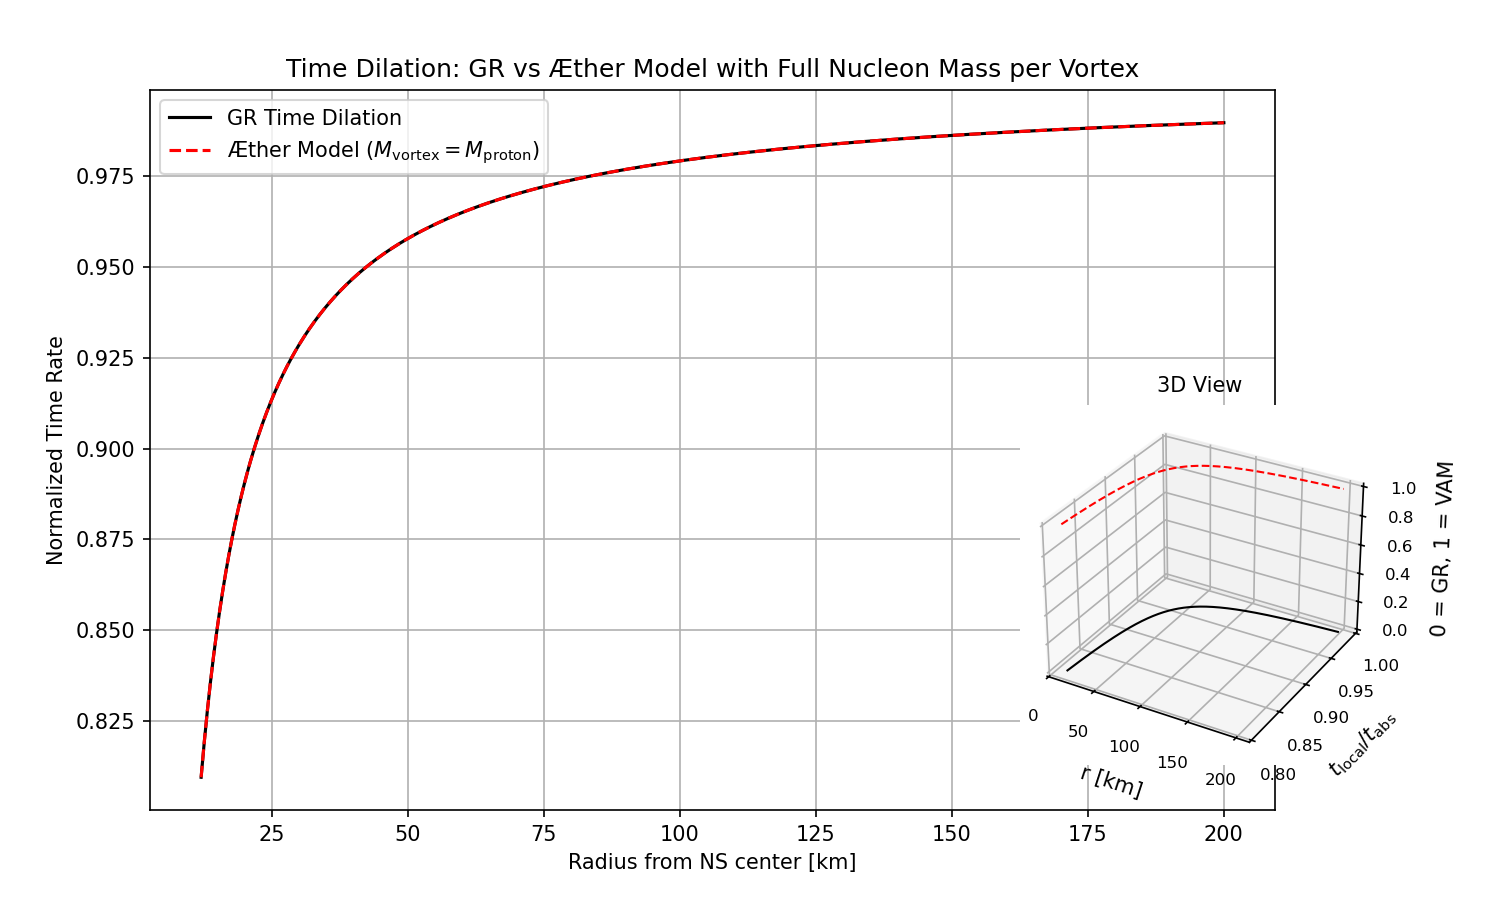
\includegraphics[width=0.85\textwidth]{images/07-TimeDilationGRVsVAM}
  \caption{
  \textbf{Comparison of Time Dilation Models:} The General Relativity (GR) time dilation formula \(\sqrt{1 - 2GM/(rc^2)}\) is contrasted with the VAM formula derived in Eq. (A1), which incorporates localized vortex angular velocity decay, vorticity-induced gravitational effects, and rotational frame dragging. The curves diverge as local rotation becomes dominant, highlighting differences in high-density regimes or vortex-based systems.
  }
  \label{fig:GRvsVAMTimeDilation}
\end{figure}



The above equation is analogous to relativistic formulas, but has a fluid mechanics origin. Experimentally, components of this formula can be found in time dilation of GPS clocks (gravity), Lense-Thirring effects (rotation), and hypothetical laboratory measurements of nuclear rotations on the quantum or vortex scale.

\section*{Conclusion}
This equation synthesizes all prior VAM elements: vortex helicity, bubble boundaries, circulation-induced gravity, and exponential suppression of short-range fields. It remains finite, matches classical predictions at macroscopic scales, and enables numerical probing at quantum scales.

\subsection{Constants and Variables}

\begin{table}[h]
      \centering
      \begin{tabular}{llll}
          \toprule
          \textbf{Symbol} & \textbf{Meaning} & \textbf{Value / Expression} & \textbf{Units} \\
          \midrule
        $G_{\text{hybrid}}(r)$ & Hybrid gravitational constant (VAM/GR) & $\mu(r) G_{\text{swirl}} + (1 - \mu(r)) G$ & $\text{m}^3\,\text{kg}^{-1}\,\text{s}^{-2}$ \\
        $\mu(r)$ & Vortex-to-classical transition function & $e^{-r^2 / R_0^2}$, $R_0 = 1.0 \times 10^{-12}\,\text{m}$ & unitless \\
        $G$ & Newtonian gravitational constant & $6.67430 \times 10^{-11}$ & $\text{m}^3\,\text{kg}^{-1}\,\text{s}^{-2}$ \\
        $G_{\text{swirl}}$ & Swirl-induced gravitational constant & $\dfrac{C_e c^5 t_p^2}{2 F_{\max} r_c^2}$ & $\text{m}^3\,\text{kg}^{-1}\,\text{s}^{-2}$ \\
        $M_{\text{hybrid}}(r)$ & Hybrid effective mass & $\mu(r) M_\text{eff}^\text{VAM}(r) + (1 - \mu(r)) M$ & $\text{kg}$ \\
        $M_\text{eff}^\text{VAM}(r)$ & Vortex effective mass & $4\pi \rho_\text{\ae} r_c^3 \left[ 2 - (2 + \frac{r}{r_c}) e^{-r/r_c} \right]$ & $\text{kg}$ \\
        $\rho_\text{\ae}$ & Æther density & $3.89343583 \times 10^{18}$ & $\text{kg}\cdot\text{m}^{-3}$ \\
        $r_c$ & Core radius (Coulomb scale) & $1.40897017 \times 10^{-15}$ & $\text{m}$ \\
        $C_e$ & Core tangential velocity & $1.09384563 \times 10^{6}$ & $\text{m}\cdot\text{s}^{-1}$ \\
        $t_p$ & Planck time & $5.391247 \times 10^{-44}$ & $\text{s}$ \\
        $F_{\max}$ & Maximum force & $29.053507$ & $\text{N}$ \\
        $\left(\frac{C_e}{r_c}\right)^2$ & Squared swirl angular frequency ($\Omega^2$) & $6.02367430 \times 10^{42}$ & $\text{s}^{-2}$ \\
        $c$ & Speed of light & $2.99792458 \times 10^8$ & $\text{m}\cdot\text{s}^{-1}$ \\
          \bottomrule
      \end{tabular}
    \caption{Key symbols and constants in the VAM time dilation equation.}
      \label{tab:time_dilation_symbols}
  \end{table}

\begin{table}
    \centering
    \begin{tabular}{llll}
        \toprule
        \textbf{Symbol} & \textbf{Meaning} & \textbf{Description} & \textbf{Value (if constant)} \\
        \midrule
        $\Delta t$ & Reference time & Clock far from gravitating body & -- \\
        $t_\text{adjusted}$ & Local time & Time experienced near the vortex structure & -- \\
        $r$ & Radial coordinate & Distance from the vortex core & m \\
        $r_c$ & Vortex core radius & Characteristic decay scale & $1.40897017 \times 10^{-15}$ m \\
        $C_e$ & Vortex tangential velocity & Maximal edge swirl velocity & $1.09384563 \times 10^6$ m/s \\
        $\rho_\text{\ae}$ & Æther density & Fluid density of the æther & $\sim 3.89 \times 10^{18}$ kg/m$^3$ \\
        $c$ & Speed of light & Vacuum light speed & $2.99792458 \times 10^8$ m/s \\
        $G$ & Newton's constant & Classical gravity & $6.67430 \times 10^{-11}$ m$^3$/kg/s$^2$ \\
        $F_{\text{max}}$ & Max force & From Planck-scale dynamics & $29.053507$ N \\
        $t_p$ & Planck time & Quantum gravity scale & $5.391247 \times 10^{-44}$ s \\
        $G_\text{swirl}$ & Vortex gravity coupling & $C_e c^5 t_p^2 / (2 F_{\text{max}} r_c^2)$ & -- \\
        $M$ & Macroscopic mass & Classical object mass (e.g., proton mass) & $1.67262192 \times 10^{-27}$ kg \\
        $M_{\text{eff}}^\text{VAM}(r)$ & VAM mass & Mass from vorticity energy & derived \\
        $M_{\text{hybrid}}(r)$ & Hybrid mass & Smooth transition between VAM and GR & -- \\
        $G_{\text{hybrid}}(r)$ & Hybrid gravity constant & Smooth transition between $G$ and $G_\text{swirl}$ & -- \\
        $\mu(r)$ & Hybrid blending function & $\mu(r) = \exp\left(-\frac{r^2}{R_0^2}\right),\ R_0 \sim 10^{-12}$ m & dimensionless \\
        $e^{-r/r_c}$ & Vorticity decay & Exponential suppression term & -- \\
        \bottomrule
    \end{tabular}
    \caption{Explanation of variables in Equation~\ref{eq:final_vam_td}.}
    \label{tab:time_dilation_variables}
\end{table}



